\documentclass[11pt,a4paper]{article}
\usepackage[margin=2.5cm]{geometry}
\usepackage[utf8]{inputenc}
\usepackage[T1]{fontenc}
\usepackage{lmodern}
\usepackage{xcolor}
\usepackage{tikz}
\usetikzlibrary{shapes.geometric, arrows.meta, positioning}
\usepackage{booktabs}
\usepackage{array}
\usepackage{colortbl}
\usepackage{multirow}
\usepackage{listings}
\usepackage[bookmarks=false]{hyperref}
\usepackage{fancyhdr}
\usepackage{amsmath}

\definecolor{fpgablue}{RGB}{13,71,161}
\definecolor{fpgalight}{RGB}{187,222,251}
\definecolor{hostgreen}{RGB}{27,94,32}
\definecolor{hostlight}{RGB}{200,230,201}
\definecolor{sigred}{RGB}{183,28,28}
\definecolor{codegray}{RGB}{248,248,248}
\definecolor{arrowgray}{RGB}{80,80,80}
\definecolor{bugred}{RGB}{220,100,100}
\definecolor{fixgreen}{RGB}{76,175,80}
\definecolor{noteyellow}{RGB}{255,249,196}
\definecolor{noteborder}{RGB}{255,193,7}
\definecolor{byteA}{RGB}{187,222,251}
\definecolor{byteB}{RGB}{200,230,201}
\definecolor{byteC}{RGB}{255,224,178}
\definecolor{byteD}{RGB}{225,190,231}
\definecolor{byteE}{RGB}{255,205,210}
\definecolor{byteG}{RGB}{232,240,254}

\tikzset{
  block/.style={rectangle, rounded corners=4pt, minimum width=2.8cm,
    minimum height=0.9cm, align=center, draw, font=\small\bfseries},
  fpgablock/.style={block, fill=fpgalight, draw=fpgablue, text=fpgablue},
  hostblock/.style={block, fill=hostlight, draw=hostgreen, text=hostgreen},
  arrow/.style={-{Stealth[length=6pt]}, thick, color=arrowgray},
  fatarrow/.style={-{Stealth[length=8pt]}, line width=2pt, color=fpgablue},
}

\pagestyle{fancy}
\fancyhf{}
\rhead{\small\textcolor{fpgablue}{FPGA Tick-to-Trade}}
\lhead{\small Part 2: RTL Design \& Verification}
\cfoot{\small\thepage}
\renewcommand{\headrulewidth}{0.5pt}

\hypersetup{colorlinks=true, linkcolor=fpgablue, urlcolor=fpgablue,
            pdftitle={FPGA Tick-to-Trade Part 2}}

\lstset{
  backgroundcolor=\color{codegray}, basicstyle=\ttfamily\footnotesize,
  keywordstyle=\color{fpgablue}\bfseries, commentstyle=\color{gray}\itshape,
  stringstyle=\color{sigred}, breaklines=true, frame=single,
  rulecolor=\color{gray!40}, numbers=left, numberstyle=\tiny\color{gray},
  xleftmargin=1.5em, xrightmargin=0.5em,
}

\begin{document}

% ── Title page ────────────────────────────────────────────────────────────────
\begin{titlepage}
\vspace*{3cm}
{\color{fpgablue}\rule{\linewidth}{2pt}}
\vspace{0.5cm}

{\fontsize{28}{34}\selectfont\bfseries\color{fpgablue} FPGA Tick-to-Trade\par}
\vspace{0.4cm}
{\Large\color{fpgablue} Part 2 --- RTL Design \& Verification\par}
\vspace{0.3cm}
{\normalsize\color{gray} Abhishek \quad\textperiodcentered\quad June 2026
  \quad\textperiodcentered\quad TESTS=81\ PASS=81\ FAIL=0\par}
\vspace{0.2cm}
{\small\itshape\color{gray}
  SystemVerilog RTL \textperiodcentered{} cocotb \textperiodcentered{}
  QuestaSim 2021.2 \textperiodcentered{} Python golden model\par}

\vspace{0.5cm}
{\color{fpgablue}\rule{\linewidth}{1pt}}
\vspace{2cm}
\tableofcontents
\end{titlepage}

% ─────────────────────────────────────────────────────────────────────────────
\section{RTL Pipeline Overview}

The five RTL modules form a strictly linear pipeline. Data flows in one direction
only; every module is clock-synchronous at the same frequency. A valid/ready
handshake between the parser and the order book provides back-pressure, so a
message arriving while the book is busy (during a rescan) is held, never dropped.

\begin{center}
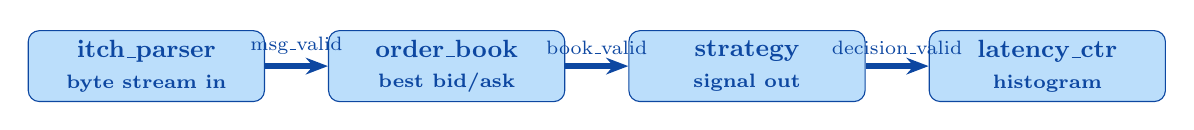
\begin{tikzpicture}[node distance=0.5cm and 0.8cm]
  \node[fpgablock, minimum width=3cm] (parser) {itch\_parser\\{\scriptsize byte stream in}};
  \node[fpgablock, right=0.8cm of parser, minimum width=3cm] (book) {order\_book\\{\scriptsize best bid/ask}};
  \node[fpgablock, right=0.8cm of book, minimum width=3cm] (strat) {strategy\\{\scriptsize signal out}};
  \node[fpgablock, right=0.8cm of strat, minimum width=3cm] (lat) {latency\_ctr\\{\scriptsize histogram}};
  \draw[fatarrow] (parser) -- (book) node[midway, above, font=\scriptsize]{msg\_valid};
  \draw[fatarrow] (book) -- (strat) node[midway, above, font=\scriptsize]{book\_valid};
  \draw[fatarrow] (strat) -- (lat) node[midway, above, font=\scriptsize]{decision\_valid};
\end{tikzpicture}
\end{center}

\noindent\textbf{Interface contract:} Every module presents data using a valid-pulse
protocol. A signal named \texttt{*\_valid} is asserted for exactly \textbf{one clock
cycle} carrying the data in that same cycle. The downstream module must be ready
to accept it (no stalling).

% ─────────────────────────────────────────────────────────────────────────────
\section{Module 1: itch\_parser.sv}

\subsection{What the Parser Does}

The parser is an \textbf{AXI-Stream slave}. It ingests one byte per clock cycle,
accumulates bytes into field shift registers, and emits a one-cycle
\texttt{m\_valid} pulse on the cycle of the last byte (\texttt{tlast}).
The outputs --- \texttt{msg\_type}, \texttt{timestamp}, \texttt{order\_ref},
\texttt{side}, \texttt{shares}, \texttt{price} --- are stable at that cycle
and held until the next \texttt{m\_valid}.

\subsection{Shift Register Accumulation}

Each multi-byte field is accumulated using a \textbf{left-shifting shift register}.
For a 64-bit \texttt{order\_ref} field spanning bytes 11--18:

\begin{lstlisting}[language=Verilog,
  caption={Left-shifting shift register: 8 bytes into 64 bits}]
// ref_sr holds the accumulated value so far
// On each byte that belongs to order_ref:
ref_sr <= {ref_sr[55:0], s_axis_tdata};  // shift left, insert new byte
\end{lstlisting}

After byte 18 the register contains the correct big-endian 64-bit value.
This requires \textbf{zero multiply, zero divide} --- just concatenation (wiring).

\subsection{ITCH 5.0 Message Byte Layouts}

Each message type is a fixed-length binary record. Byte 0 is always the message
type character (ASCII). The parser routes subsequent bytes using
\texttt{case(byte\_cnt)}.

\vspace{0.6em}
\noindent\textbf{Add Order (A) --- 36 bytes}

\begin{center}
\small
\begin{tabular}{c c l}
\toprule
\textbf{Bytes} & \textbf{Field} & \textbf{Notes} \\
\midrule
0      & msg\_type  & 0x41 = 'A' \\
1--2   & stock\_locate & 2B big-endian \\
3--4   & tracking\_number & 2B \\
5--10  & timestamp  & 6B nanoseconds \\
11--18 & order\_ref & 8B unique ID \\
19     & side       & 'B'=bid, 'S'=ask \\
20--23 & shares     & 4B \\
24--31 & stock      & 8B symbol (ignored) \\
32--35 & price      & 4B fixed-point $\times$10{,}000 \\
\bottomrule
\end{tabular}
\end{center}

\vspace{0.6em}
\noindent\textbf{Cancel (X) --- 23 bytes} \quad and \quad \textbf{Delete (D) --- 19 bytes}

\begin{center}
\small
\begin{tabular}{c c l l}
\toprule
\textbf{Bytes} & \textbf{Field} & \textbf{Cancel (X)} & \textbf{Delete (D)} \\
\midrule
0      & msg\_type  & 0x58 & 0x44 \\
1--4   & locate/tracking & same & same \\
5--10  & timestamp  & same & same \\
11--18 & order\_ref & bytes 11--18, \texttt{tlast}=byte 18 & bytes 11--18, \texttt{tlast}=byte 18 \\
19--22 & cancelled shares & 4B (Cancel only) & --- \\
\bottomrule
\end{tabular}
\end{center}

\noindent\textit{Key observation:} For Cancel and Delete, the last parsed field
(\texttt{order\_ref}) ends on the same byte as \texttt{tlast}. This is the root
cause of the NBA timing bug described in Section~\ref{sec:nba}.

\subsection{Parser State Machine}

\begin{center}
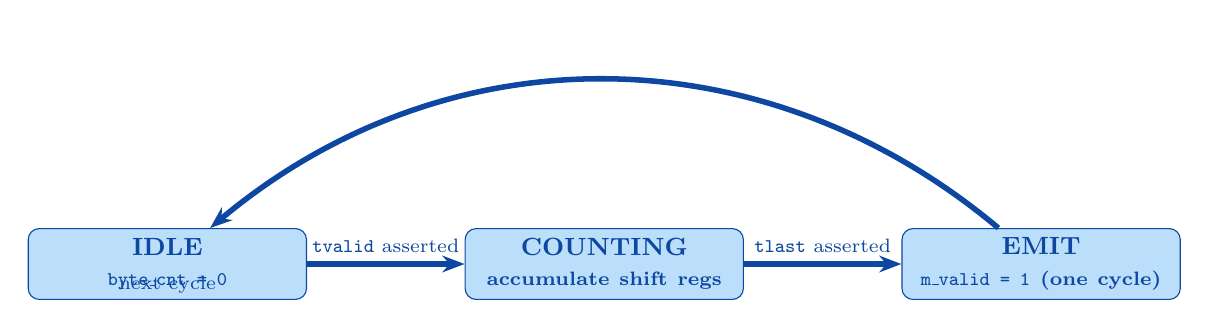
\begin{tikzpicture}[node distance=1.5cm]
  \node[fpgablock, minimum width=3.5cm, text width=3.3cm] (idle)
    {IDLE\\{\scriptsize \texttt{byte\_cnt = 0}}};
  \node[fpgablock, right=2cm of idle, minimum width=3.5cm, text width=3.3cm] (count)
    {COUNTING\\{\scriptsize accumulate shift regs}};
  \node[fpgablock, right=2cm of count, minimum width=3.5cm, text width=3.3cm] (emit)
    {EMIT\\{\scriptsize \texttt{m\_valid = 1} (one cycle)}};
  \draw[fatarrow] (idle) -- (count)
    node[midway, above, font=\scriptsize]{\texttt{tvalid} asserted};
  \draw[fatarrow] (count) -- (emit)
    node[midway, above, font=\scriptsize]{\texttt{tlast} asserted};
  \draw[fatarrow] (emit) to[bend right=40] (idle)
    node[midway, below, font=\scriptsize]{next cycle};
\end{tikzpicture}
\end{center}

In COUNTING state, \texttt{byte\_cnt} increments on each \texttt{tvalid} cycle.
A \texttt{case(byte\_cnt)} routes each byte to its field shift register using
\texttt{always\_comb} (\texttt{\_nxt} wires). On \texttt{tlast}: outputs latch
the \texttt{\_nxt} values.

\subsection{Critical Bug: Non-Blocking Assignment Timing}
\label{sec:nba}

\subsubsection{What Are Non-Blocking Assignments?}

In SystemVerilog, \texttt{always\_ff} blocks use the non-blocking assignment
operator (\texttt{<=}). The IEEE 1800 standard defines two phases per clock edge:

\begin{enumerate}
  \item \textbf{Active region:} Right-hand sides of all \texttt{<=} assignments
    are evaluated using the \emph{current} (pre-edge) values of all signals.
  \item \textbf{NBA region:} The computed values are written to the registers.
\end{enumerate}

This means: if \texttt{A <= B + 1} and \texttt{C <= A}, both use the \textbf{old}
value of \texttt{A}. This is correct and intentional for pipelined RTL --- but it
creates a subtle trap when capturing a signal on the same cycle it is being updated.

\subsubsection{The Bug}

When the last byte of \texttt{order\_ref} (byte 18) arrives on the same cycle
as \texttt{tlast}, the \texttt{always\_ff} block evaluates
\texttt{order\_ref <= ref\_sr} using the \emph{pre-edge} value of \texttt{ref\_sr}
(bytes 11--17 only). Byte 18 was just presented to the shift register on that
edge --- it will be in \texttt{ref\_sr} only \emph{after} the NBA update, one
cycle later. The output \texttt{order\_ref} is therefore missing the last byte.

\begin{center}
\small
\begin{tabular}{l l l}
\toprule
\textbf{Signal} & \textbf{At \texttt{tlast} rising edge} & \textbf{Effect} \\
\midrule
\texttt{ref\_sr}   & holds bytes 11--17 (pre-edge) & NBA not yet applied \\
\rowcolor{bugred!15}
\texttt{order\_ref} (BUG) & captures \texttt{ref\_sr} = bytes 11--17 & missing byte 18! \\
\rowcolor{fixgreen!15}
\texttt{order\_ref} (FIX) & captures \texttt{ref\_nxt} = bytes 11--18 & correct \\
\bottomrule
\end{tabular}
\end{center}

\subsubsection{The Fix: Combinational \_nxt Wires}

Add an \texttt{always\_comb} block that computes the \emph{next} value of each
shift register including the \emph{current} byte. The \texttt{always\_ff} block
then uses these \texttt{\_nxt} signals for both the register update and the output latch:

\begin{lstlisting}[language=Verilog,
  caption={Combinational \_nxt fix --- the core pattern in itch\_parser.sv}]
// COMBINATIONAL: compute next-state shift register values
// This sees s_axis_tdata (the CURRENT byte) right now.
always_comb begin
    ref_nxt = ref_sr;           // default: hold
    if (tvalid && tready) begin
        case (byte_cnt)
            6'd11, 6'd12, 6'd13, 6'd14,
            6'd15, 6'd16, 6'd17, 6'd18:
                ref_nxt = {ref_sr[55:0], s_axis_tdata};  // include current byte
        endcase
    end
end

// SEQUENTIAL: on clock edge, use _nxt (not _sr)
always_ff @(posedge clk or negedge rst_n) begin
    if (!rst_n) begin
        ref_sr    <= '0;
        order_ref <= '0;
        m_valid   <= 1'b0;
    end else begin
        ref_sr  <= ref_nxt;          // normal pipeline update
        m_valid <= 1'b0;             // default: deassert
        if (s_axis_tlast) begin
            order_ref <= ref_nxt;    // FIX: _nxt includes the current byte
            m_valid   <= 1'b1;       // one-cycle pulse
        end
    end
end
\end{lstlisting}

The \texttt{always\_comb} block is combinational logic --- it evaluates
instantaneously. Because it includes \texttt{s\_axis\_tdata} on the right-hand
side, \texttt{ref\_nxt} already contains the correct shifted value before the
clock edge arrives. The \texttt{always\_ff} block then latches \texttt{ref\_nxt},
not the stale \texttt{ref\_sr}.

\subsection{Tests that Failed and Why}

\begin{center}
\small
\begin{tabular}{l l l c l}
\toprule
\textbf{Test} & \textbf{Msg} & \textbf{Last field ends at} & \textbf{= tlast?} & \textbf{Pre-fix} \\
\midrule
\rowcolor{bugred!18}
\texttt{test\_add\_order}     & Add (36B)    & price byte 35      & YES & FAIL \\
\rowcolor{fixgreen!18}
\texttt{test\_sell\_add}      & Add (36B)    & side byte 19       & no  & PASS \\
\rowcolor{bugred!18}
\texttt{test\_cancel}         & Cancel (23B) & shares byte 22     & YES & FAIL \\
\rowcolor{bugred!18}
\texttt{test\_delete}         & Delete (19B) & order\_ref byte 18 & YES & FAIL \\
\rowcolor{fixgreen!18}
\texttt{test\_execute}        & Execute (31B) & shares byte 22    & no (last=30) & PASS \\
\rowcolor{bugred!18}
\texttt{test\_back\_to\_back} & mixed        & ---                & ---          & FAIL \\
\bottomrule
\end{tabular}
\end{center}

\noindent Tests fail when the \emph{last byte of the last captured field} coincides
with \texttt{tlast}. The \texttt{\_nxt} fix resolves all six cases.

% ─────────────────────────────────────────────────────────────────────────────
\section{Module 2: order\_book\_top.sv}

\subsection{Why Order Book Reconstruction?}

A raw ITCH feed does not tell you the current price. It only tells you what
\emph{happened}: ``order 1234 was added at \$150.01 for 500 shares.''
To know the best available bid and ask at any moment, you must maintain a
\textbf{limit order book}: a data structure that tracks all live orders and
exposes the best (highest bid, lowest ask) at all times.

\subsection{Milestone 1 Data Structure: Direct-Mapped Register File}

The order book is implemented as a \textbf{256-entry register file}, directly
indexed by the low 8 bits of the 64-bit \texttt{order\_ref} number.

\begin{center}
\small
\begin{tabular}{l l}
\toprule
\textbf{Field} & \textbf{Width / Notes} \\
\midrule
\texttt{valid}     & 1 bit --- 1 = live order in this slot \\
\texttt{order\_ref} & 64 bits --- full reference number \\
\texttt{side}      & 1 bit --- 0=BID, 1=ASK \\
\texttt{price}     & 32 bits --- fixed-point $\times$10{,}000 \\
\texttt{shares}    & 32 bits --- remaining shares \\
\midrule
Index & \texttt{order\_ref[7:0]} --- direct map, O(1) lookup \\
\bottomrule
\end{tabular}
\end{center}

\noindent\textbf{Why direct-mapped?} O(1) lookup with no comparator chain.
No sorting, no priority encoding required. \texttt{order\_book\_m2} extends this
into a \textbf{multi-level} structure that tracks the top 4 price levels per side
(price + aggregated size), while keeping the Add path O(1) (see Section on the
RESCAN FSM).

\noindent\textbf{Struct definition:}
\begin{lstlisting}[language=Verilog, caption={Order entry typedef in order\_book\_top.sv}]
typedef struct packed {
    logic        valid;          // 1 = this slot has a live order
    logic [63:0] order_ref;      // full 64-bit order reference number
    logic        side;           // 0=BID, 1=ASK
    logic [31:0] price;          // price * 10,000 (fixed-point)
    logic [31:0] shares;         // remaining shares
} order_entry_t;

order_entry_t entries [0:ORDER_DEPTH-1];  // 256 entries
\end{lstlisting}

\subsection{Message Processing}

\begin{center}
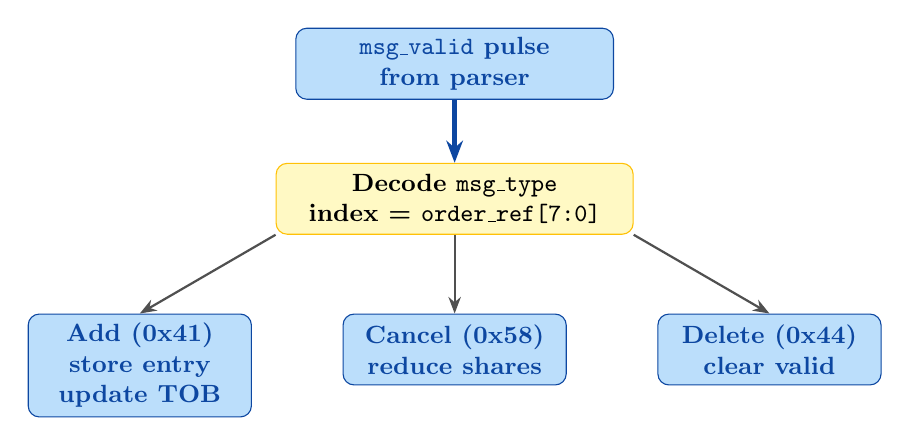
\begin{tikzpicture}[node distance=1.2cm]
  \node[fpgablock, minimum width=4cm, text width=3.8cm]
    (msg) {\texttt{msg\_valid} pulse\\from parser};
  \node[block, fill=noteyellow, draw=noteborder, below=0.8cm of msg,
        minimum width=4.5cm, text width=4.3cm]
    (type) {Decode \texttt{msg\_type}\\index = \texttt{order\_ref[7:0]}};
  \node[fpgablock, below left=1cm and 0.3cm of type,
        minimum width=2.8cm, text width=2.6cm]
    (add) {Add (0x41)\\store entry\\update TOB};
  \node[fpgablock, below=1cm of type,
        minimum width=2.8cm, text width=2.6cm]
    (cancel) {Cancel (0x58)\\reduce shares};
  \node[fpgablock, below right=1cm and 0.3cm of type,
        minimum width=2.8cm, text width=2.6cm]
    (del) {Delete (0x44)\\clear valid};
  \draw[fatarrow] (msg) -- (type);
  \draw[arrow] (type.south west) -- (add.north);
  \draw[arrow] (type) -- (cancel);
  \draw[arrow] (type.south east) -- (del.north);
\end{tikzpicture}
\end{center}

\noindent\textit{M1 limitation:} best bid/ask is NOT re-scanned after
cancel/delete. This is the central problem solved in Milestone~2
(Section~\ref{sec:m2book}).

\subsection{Known Bug Fixed: table is a Reserved Keyword}

SystemVerilog reserves the keyword \texttt{table} for UDP (User-Defined
Primitive) truth tables. Using it as a variable name causes a parse error:

\begin{center}
\small
\begin{tabular}{l l}
\toprule
\textbf{Original (broken)} & \textbf{Fixed} \\
\midrule
\texttt{order\_entry\_t table [...];} & \texttt{order\_entry\_t entries [...];} \\
\bottomrule
\end{tabular}
\end{center}

% ─────────────────────────────────────────────────────────────────────────────
\section{Module 2b: order\_book\_m2.sv --- The RESCAN FSM}
\label{sec:m2book}

\subsection{The Stale-Best Problem}

Milestone~1's order book is correct \emph{only} for Add messages. When an order
is cancelled, deleted, or partially executed, M1 updates the stored entry but
\textbf{never re-examines the best bid/ask}. Consider this sequence:

\begin{center}
\small
\begin{tabular}{l l l l}
\toprule
\textbf{Step} & \textbf{Message} & \textbf{M1 best\_bid} & \textbf{Correct best\_bid} \\
\midrule
1 & Add ref=1 bid \$100 $\times$50 & \$100 $\times$50 & \$100 $\times$50 \\
2 & Add ref=2 bid \$90 $\times$30  & \$100 $\times$50 & \$100 $\times$50 \\
\rowcolor{bugred!18}
3 & Delete ref=1 (the \$100 bid)   & \$100 $\times$50 \textit{(stale!)} & \$90 $\times$30 \\
\bottomrule
\end{tabular}
\end{center}

\noindent After step 3 the \$100 order is gone, yet M1 still reports it as the
best bid. A strategy reading this would trade on a price that no longer exists ---
in HFT terms, a \textbf{phantom quote}. M2 fixes this.

\subsection{Design: A Two-State FSM with a Single-Pass Rescan}

The fix is conceptually simple: after any Cancel/Delete/Execute, re-scan
\emph{all} 256 entries and recompute the best bid and ask from scratch. The
challenge is doing it in hardware without a comparator tree across 256 entries
(which would never meet timing at 200\,MHz). The solution is to \textbf{spread
the scan over time}: one entry per clock cycle, using a small FSM.

\begin{center}
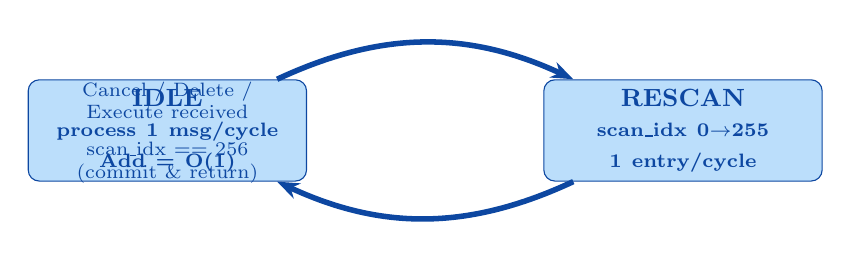
\begin{tikzpicture}[node distance=2.2cm]
  \node[fpgablock, minimum width=3.5cm, text width=3.3cm]
    (idle) {\textbf{IDLE}\\{\scriptsize process 1 msg/cycle}\\{\scriptsize Add = O(1)}};
  \node[fpgablock, right=3cm of idle, minimum width=3.5cm, text width=3.3cm]
    (rescan) {\textbf{RESCAN}\\{\scriptsize scan\_idx 0$\to$255}\\{\scriptsize 1 entry/cycle}};
  \draw[fatarrow] (idle) to[bend left=25] (rescan)
    node[midway, above, font=\scriptsize, align=center]{Cancel / Delete /\\Execute received};
  \draw[fatarrow] (rescan) to[bend left=25] (idle)
    node[midway, below, font=\scriptsize, align=center]{scan\_idx == 256\\(commit \& return)};
\end{tikzpicture}
\end{center}

\noindent\textbf{Add path is untouched} --- it stays O(1) in the IDLE state,
exactly as in M1. Only the destructive messages (C/D/E) pay the rescan cost.
This matters: Add is by far the most common message in a real feed, so the
common case stays single-cycle.

\subsection{The Single-Pass Best-of-N Algorithm}

During RESCAN, the FSM keeps running accumulators (\texttt{scan\_bid\_p/s},
\texttt{scan\_ask\_p/s}). At each entry it applies the classic
\emph{find-max-in-one-pass} rule, extended to also \textbf{aggregate size at the
winning price}:

\begin{lstlisting}[language=Verilog,
  caption={Per-entry rescan logic --- bid side (ask is the mirror with \texttt{<})}]
if (entries[scan_idx].valid && !entries[scan_idx].side) begin   // a bid
    if (!scan_bid_seen || entries[scan_idx].price > scan_bid_p) begin
        // strictly better price: start a fresh best level
        scan_bid_p    <= entries[scan_idx].price;
        scan_bid_s    <= entries[scan_idx].shares;
        scan_bid_seen <= 1'b1;
    end else if (entries[scan_idx].price == scan_bid_p) begin
        // same price as current best: add this order's shares to the level
        scan_bid_s <= scan_bid_s + entries[scan_idx].shares;
    end
    // worse price: ignore
end
\end{lstlisting}

\noindent For the ask side the only change is \texttt{<} instead of \texttt{>}
(lowest ask wins). When \texttt{scan\_idx} reaches 256, the accumulated values
are committed to the output registers and the FSM returns to IDLE.

\subsection{The Off-by-One Trap: Why the Scan Runs 257 Cycles}

A 256-entry table needs \textbf{257} cycles, not 256. This is the same NBA
subtlety from Section~\ref{sec:nba}, now on the read side. When the FSM examines
the last entry (\texttt{scan\_idx == 255}), the accumulator update is a
non-blocking assignment --- it does not take effect until the \emph{next} clock
edge. If we committed on the cycle \texttt{scan\_idx == 255}, we would read the
accumulators \emph{before} entry 255 was folded in, silently dropping the last
order.

\begin{center}
\small
\begin{tabular}{c l l}
\toprule
\textbf{Cycle} & \textbf{Action} & \textbf{State of accumulators} \\
\midrule
0--254 & scan entries 0--254 & folding each entry in \\
255    & scan entry 255      & entry 255's NBA \emph{scheduled}, not yet visible \\
\rowcolor{fpgalight}
256    & \texttt{scan\_idx == 256}: COMMIT & entry 255's NBA now settled --- read safely \\
\bottomrule
\end{tabular}
\end{center}

\noindent The extra commit cycle is why \texttt{scan\_idx} is declared
\texttt{[ADDR\_W:0]} (9 bits, reaching 256) rather than \texttt{[ADDR\_W-1:0]}
(8 bits, wrapping at 255). \textbf{The same NBA rule bites twice in this project}
--- once writing (parser), once reading (rescan commit).

\subsection{The Cost, and the Optimisations Now Applied}

A worst-case RESCAN takes 257 cycles $\times$ 5\,ns $=$ \textbf{1.285\,$\mu$s} at
200\,MHz. Two optimisations (both now implemented) keep this off the critical
path in the common case:

\begin{center}
\small
\begin{tabular}{l l l}
\toprule
\textbf{Concern} & \textbf{Original M2} & \textbf{Now (implemented)} \\
\midrule
Best after C/D/E      & \textcolor{fixgreen}{correct (rescan)} & \textcolor{fixgreen}{correct} \\
Add latency           & \textcolor{fixgreen}{1 cycle} & \textcolor{fixgreen}{1 cycle} \\
Msgs during rescan    & \textcolor{sigred}{dropped} & \textcolor{fixgreen}{held (\texttt{msg\_ready} backpressure)} \\
Rescan trigger        & every C/D/E & \textcolor{fixgreen}{only if a \emph{displayed} level is touched} \\
\bottomrule
\end{tabular}
\end{center}

\noindent\textbf{Back-pressure:} the book asserts \texttt{msg\_ready} only in
IDLE; the parser holds \texttt{m\_valid} (and stalls its byte input) until the
book accepts, so nothing is dropped during a rescan. \textbf{Selective rescan:}
a Cancel/Delete/Execute on an order priced \emph{beyond the tracked depth}
cannot change any shown level, so it skips the rescan entirely and only updates
the full-depth order table. Correctness first (obvious full rescan), then these
two safe optimisations on top.

\subsection{Verification --- tb\_order\_book\_m2.py (28/28 PASS)}

The M2 testbench targets exactly the behaviours M1 got wrong. The
\textbf{headline test} drives the stale-best sequence from the top of this
section and asserts the corrected result:

\begin{lstlisting}[language=Python,
  caption={The test that proves M2 fixes the phantom quote}]
async def test_delete_best_bid_reveals_second(dut):
    await drive_msg(dut, ADD, order_ref=1, side=BID, shares=50, price=1000_0000)
    await drive_msg(dut, ADD, order_ref=2, side=BID, shares=30, price=900_0000)
    check(dut, bid_p=1000_0000, bid_s=50, tag="before delete")

    await drive_msg(dut, DELETE, order_ref=1, side=BID, shares=0, price=0)
    await wait_rescan(dut)                      # wait out the 257-cycle FSM
    check(dut, bid_p=900_0000, bid_s=30, tag="after delete best bid")  # M1 fails here
\end{lstlisting}

\begin{center}
\small
\begin{tabular}{l p{8.2cm} c}
\toprule
\textbf{Test} & \textbf{What it proves} & \textbf{Status} \\
\midrule
\rowcolor{fixgreen!12}
delete\_best\_bid\_reveals\_second & deleting the best bid promotes the 2nd-best & PASS \\
\rowcolor{fixgreen!12}
delete\_non\_best\_bid\_unchanged  & deleting a lower bid leaves best intact & PASS \\
\rowcolor{fixgreen!12}
cancel\_partial\_reduces\_size     & partial cancel updates size after rescan & PASS \\
\rowcolor{fixgreen!12}
cancel\_full\_empties\_book        & removing last order drops book\_valid to 0 & PASS \\
\rowcolor{fixgreen!12}
execute\_reduces\_size             & execute decrements remaining shares & PASS \\
\rowcolor{fixgreen!12}
two\_asks\_delete\_best\_reveals\_higher & ask side mirror of the bid test & PASS \\
\rowcolor{fixgreen!12}
aggregate\_then\_partial\_cancel   & size aggregation survives a partial cancel & PASS \\
\midrule
\multicolumn{2}{r}{\bfseries + basic Add/level, replace, rescan-skip, AXI tests \quad TOTAL} & 28/28 \\
\bottomrule
\end{tabular}
\end{center}

\noindent\textbf{Hash-collision gotcha:} the table is indexed by
\texttt{order\_ref[7:0]}, so \texttt{order\_ref=1} and \texttt{order\_ref=257}
map to the \emph{same} slot. Early test drafts used 257 as a ``second order''
and silently overwrote the first. Tests now use small, distinct refs
(1, 2, 10, 11) that occupy different slots.

% ─────────────────────────────────────────────────────────────────────────────
\section{Module 3: strategy\_imbalance.sv}

\subsection{The Book Imbalance Signal}

Book imbalance is a well-known short-term price predictor in market microstructure.
The observable bid-ask imbalance is a proxy signal for informed order flow:

\[
\text{Imbalance} = \frac{\text{bid\_size}}{\text{bid\_size} + \text{ask\_size}}
\in [0, 1]
\]

A value near 1 means bid is dominant (buyers outnumber sellers)
$\Rightarrow$ price likely to rise $\Rightarrow$ \textbf{BUY} signal.
A value near 0 means ask is dominant $\Rightarrow$ \textbf{SELL} signal.

\noindent The core test below uses the top-of-book sizes for clarity; the shipped
strategy generalises this to a \emph{depth-weighted} volume over the top 4 levels
and adds a spread guard, a post-trade cooldown and imbalance-scaled lot sizing
(see Section~\ref{sec:m2add}, Milestone 2 Feature Additions).

\subsection{Fixed-Point Cross-Multiply Implementation}

Division is implemented as cross-multiplication to avoid any floating-point unit
or multi-cycle divider:

\begin{center}
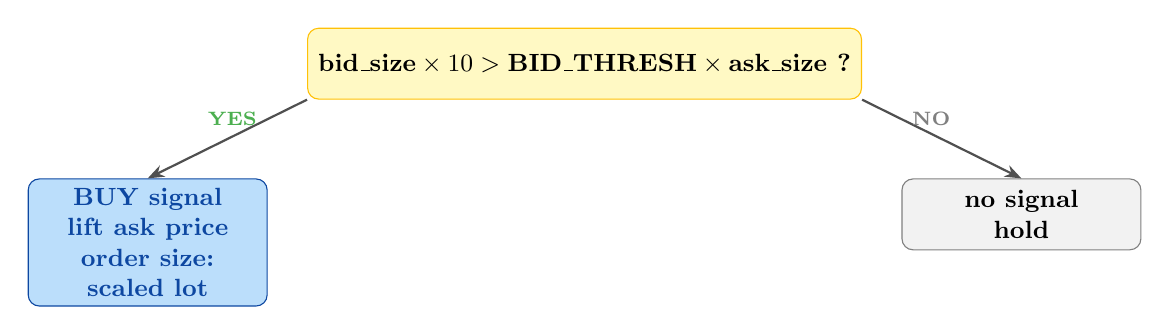
\begin{tikzpicture}[node distance=1.2cm]
  \node[block, fill=noteyellow, draw=noteborder,
        minimum width=7cm, text width=6.8cm]
    (cond) {$\text{bid\_size} \times 10 > \text{BID\_THRESH} \times \text{ask\_size}$ ?};
  \node[fpgablock, below left=1cm and 0.5cm of cond,
        minimum width=3cm, text width=2.8cm]
    (buy) {BUY signal\\lift ask price\\order size: scaled lot};
  \node[block, fill=gray!10, draw=gray, below right=1cm and 0.5cm of cond,
        minimum width=3cm, text width=2.8cm]
    (hold) {no signal\\hold};
  \draw[arrow] (cond.south west) -- (buy.north)
    node[near start, left, font=\scriptsize\bfseries]{\textcolor{fixgreen}{YES}};
  \draw[arrow] (cond.south east) -- (hold.north)
    node[near start, right, font=\scriptsize\bfseries]{\textcolor{gray}{NO}};
\end{tikzpicture}
\end{center}

\noindent\textbf{Default parameter:} \texttt{BID\_THRESH = 15} corresponds to
$\frac{15}{10} = 1.5\times$. The bid must be at least 1.5$\times$ larger than
the ask (by share count) to trigger a BUY. One DSP block per side.
One clock cycle, no division.

% ─────────────────────────────────────────────────────────────────────────────
\section{Module 4: latency\_counter.sv}

\subsection{Why Hardware Latency Measurement?}

Software timing using \texttt{clock\_gettime()} has a resolution of
$\sim$1\,$\mu$s and adds measurement jitter. A hardware counter with a 5\,ns
clock period can measure latency to \textbf{single-cycle precision}.

The counter architecture:
\begin{itemize}
  \item A free-running 32-bit counter increments every clock cycle
  \item \texttt{t0} is captured when the AXI-Stream \texttt{tvalid} rises
  \item \texttt{t1 - t0} (the \emph{delta}) is computed when \texttt{decision\_valid} fires
  \item The delta is binned into a 64-bucket BRAM histogram (bucket = delta / 4 cycles)
\end{itemize}

\begin{center}
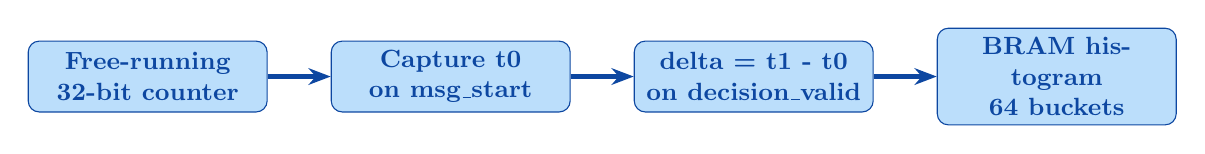
\begin{tikzpicture}[node distance=0.8cm]
  \node[fpgablock, minimum width=3cm, text width=2.8cm]
    (cnt) {Free-running\\32-bit counter};
  \node[fpgablock, right=0.8cm of cnt, minimum width=3cm, text width=2.8cm]
    (t0) {Capture t0\\on msg\_start};
  \node[fpgablock, right=0.8cm of t0, minimum width=3cm, text width=2.8cm]
    (t1) {delta = t1 - t0\\on decision\_valid};
  \node[fpgablock, right=0.8cm of t1, minimum width=3cm, text width=2.8cm]
    (hist) {BRAM histogram\\64 buckets};
  \draw[fatarrow] (cnt) -- (t0);
  \draw[fatarrow] (t0) -- (t1);
  \draw[fatarrow] (t1) -- (hist);
\end{tikzpicture}
\end{center}

\subsection{Ideal Histogram: Single Spike}

On an FPGA, every identical message takes the same number of cycles.
The ideal histogram has a \textbf{single bin} with count = number of messages:

\begin{center}
\small
\begin{tabular}{l c l}
\toprule
\textbf{Latency bucket} & \textbf{Count} & \textbf{Note} \\
\midrule
0--16\,ns (buckets 0--3)   & 0   & below pipeline latency \\
\rowcolor{fpgalight}
\textbf{20\,ns (bucket 5)} & \textbf{100} & all 100 messages land here --- single spike \\
24--48\,ns (buckets 6--12) & 0   & no jitter above baseline \\
\bottomrule
\end{tabular}
\end{center}

\noindent Every message takes exactly 20\,ns (5 buckets at 200\,MHz).
A CPU would show a distribution spanning 3--4 orders of magnitude.
This single spike is the visual proof of hardware determinism.

% ─────────────────────────────────────────────────────────────────────────────
\section{Module 5: tick\_to\_trade\_top.sv}

The top-level wrapper instantiates all four modules and wires the inter-module
signals. It packages the trading decision into a single 72-bit bus:

\begin{center}
\small
\begin{tabular}{l l l}
\toprule
\textbf{Bits} & \textbf{Signal} & \textbf{Description} \\
\midrule
{[71:65]} & reserved (7'b0)    & padding to 72-bit boundary \\
{[64]}    & \texttt{action}     & 0 = BUY, 1 = SELL \\
{[63:32]} & \texttt{order\_price} & limit price (fixed-point $\times$10{,}000) \\
{[31:0]}  & \texttt{order\_size}  & number of shares (default 100) \\
\bottomrule
\end{tabular}
\end{center}

\noindent This bus is read by the EC2 host via PCIe DMA, decoded, and passed to
\texttt{ibkr\_bridge.py}.

% ─────────────────────────────────────────────────────────────────────────────
\section{Verification Framework}

\subsection{Why Golden Model Comparison?}

A ``golden model'' is a functionally correct reference implementation in Python.
Instead of writing expected values by hand (error-prone for complex protocols),
the testbench:
\begin{enumerate}
  \item Generates the same test vector for both RTL and the golden model
  \item Runs both in parallel
  \item Asserts that every output field matches bit-for-bit
\end{enumerate}

\begin{center}
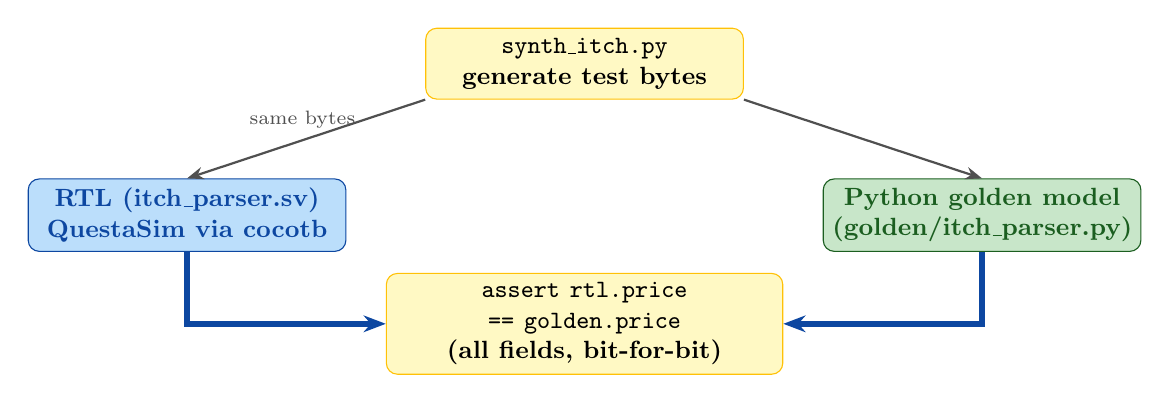
\begin{tikzpicture}[node distance=1cm]
  \node[block, fill=noteyellow, draw=noteborder, minimum width=4cm, text width=3.8cm]
    (synth) {\texttt{synth\_itch.py}\\generate test bytes};
  \node[fpgablock, below left=1cm and 1cm of synth, minimum width=4cm, text width=3.8cm]
    (rtl) {RTL (itch\_parser.sv)\\QuestaSim via cocotb};
  \node[hostblock, below right=1cm and 1cm of synth, minimum width=4cm, text width=3.8cm]
    (golden) {Python golden model\\(golden/itch\_parser.py)};
  \node[block, fill=noteyellow, draw=noteborder, below=2.2cm of synth,
        minimum width=5cm, text width=4.8cm]
    (cmp) {\texttt{assert rtl.price == golden.price}\\(all fields, bit-for-bit)};
  \draw[arrow] (synth.south west) -- (rtl.north)
    node[near start, left, font=\scriptsize]{same bytes};
  \draw[arrow] (synth.south east) -- (golden.north);
  \draw[fatarrow] (rtl.south) |- (cmp.west);
  \draw[fatarrow] (golden.south) |- (cmp.east);
\end{tikzpicture}
\end{center}

\subsection{The cocotb-Side NBA Trap: Reading Registered Outputs}
\label{sec:cocotbnba}

Section~\ref{sec:nba} described the NBA rule \emph{inside} the RTL. The same rule
bites in the \textbf{Python testbench}, and it is the single most common cocotb
mistake. After \texttt{await RisingEdge(dut.clk)}, cocotb resumes in the
\textbf{Active region} --- \emph{before} Questa has committed that edge's
non-blocking assignments. So a registered output you expect to have just changed
still shows its \emph{old} value.

\begin{center}
\small
\begin{tabular}{l p{9cm}}
\toprule
\textbf{Symptom} & \textbf{Cause} \\
\midrule
\rowcolor{bugred!15}
Output reads 0 right after driving an input &
  \texttt{always\_ff} fired, but its \texttt{<=} has not committed when cocotb
  reads in the Active region of the same edge \\
\bottomrule
\end{tabular}
\end{center}

\noindent\textbf{The fix} is to wait one \emph{additional} \texttt{RisingEdge}
after the edge that triggers the update, letting the NBA settle into the Active
region of the following cycle. Every driver helper in this project bakes this in:

\begin{lstlisting}[language=Python,
  caption={The two-edge \texttt{drive\_msg} pattern (used in every order-book test)}]
async def drive_msg(dut, msg_type, order_ref, side, shares, price):
    dut.msg_valid.value = 1
    dut.msg_type.value  = msg_type
    # ... drive the rest of the inputs ...
    await RisingEdge(dut.clk)   # always_ff fires; NBAs are SCHEDULED
    dut.msg_valid.value = 0
    await RisingEdge(dut.clk)   # NBAs from the previous edge now COMMITTED -> safe to read
\end{lstlisting}

\noindent The integration test hit a two-deep version of this: the strategy sets
\texttt{decision\_valid} at edge $T$, the latency counter reacts at $T{+}1$, so
\texttt{last\_latency\_cycles} is only valid at $T{+}2$. The fix is to capture
\texttt{m\_axis\_tdata} immediately on seeing \texttt{tvalid}, then
\texttt{await} one more edge before reading the latency. \textbf{Rule of thumb:}
one extra \texttt{RisingEdge} per pipeline register between the input you drove
and the output you read.

\subsection{Test Results --- 81/81 PASS}

The suite spans six testbenches across both order-book generations, every output
diffed bit-for-bit against the Python golden model; all RTL is
\texttt{verilator -Wall} lint-clean:

\begin{center}
\small
\begin{tabular}{l l c l}
\toprule
\textbf{Testbench} & \textbf{DUT} & \textbf{Result} & \textbf{Focus} \\
\midrule
\rowcolor{fixgreen!12}
tb\_itch\_parser.py        & itch\_parser.sv        & 11/11 & 8 msg types, back-to-back, back-pressure hold \\
\rowcolor{fixgreen!12}
tb\_order\_book.py         & order\_book\_top.sv    & 11/11 & M1 top-of-book on Add \\
\rowcolor{fixgreen!12}
tb\_order\_book\_m2.py     & order\_book\_m2.sv     & 28/28 & multi-level, RESCAN, replace, rescan-skip \\
\rowcolor{fixgreen!12}
tb\_strategy\_imbalance.py & strategy\_imbalance.sv & 21/21 & spread guard, cooldown, lot tiers, depth weight \\
\rowcolor{fixgreen!12}
tb\_latency\_counter.py    & latency\_counter.sv    & 5/5   & histogram, saturation, AXI-Lite read, clear \\
\rowcolor{fixgreen!12}
tb\_tick\_to\_trade.py     & tick\_to\_trade\_top.sv & 5/5  & end-to-end 195\,ns, back-pressure no-drop \\
\midrule
\multicolumn{2}{r}{\bfseries TESTS=81\ \ PASS=81\ \ FAIL=0} & \textbf{81/81} & \\
\bottomrule
\end{tabular}
\end{center}

\noindent\textbf{Headline number:} the integration test measures a
hardware-counted tick-to-trade latency of \textbf{39 cycles = 195\,ns} at
200\,MHz for an Add Order --- 36 parser cycles $+$ 1 book $+$ 2 strategy gate.

\subsection{Issues Log}

\begin{center}
\small
\begin{tabular}{p{3.0cm} p{4.2cm} p{5.5cm}}
\toprule
\textbf{Issue} & \textbf{Root Cause} & \textbf{Fix Applied} \\
\midrule
\texttt{table} syntax error &
  Reserved SV keyword (UDP truth tables) &
  Renamed array to \texttt{entries} \\
\addlinespace
\texttt{timescale} error in Questa &
  Questa 2021.2 + \texttt{-mfcu}: per-file timescale mis-parsed &
  Removed from all RTL; added \texttt{-timescale 1ns/1ps} to Makefile \\
\addlinespace
Wrong price / shares / order\_ref &
  NBA timing: last field byte and \texttt{tlast} same cycle &
  Combinational \texttt{\_nxt} wires; outputs use \texttt{\_nxt} at \texttt{tlast} \\
\addlinespace
Back-to-back test timeout &
  \texttt{collect\_output} missed the one-cycle \texttt{m\_valid} pulse &
  Parallel \texttt{monitor()} coroutine checks immediately \\
\addlinespace
\texttt{units=} deprecation &
  cocotb 2.x renamed \texttt{units=} to \texttt{unit=} in \texttt{Clock()} &
  Updated all \texttt{Clock()} calls \\
\addlinespace
Output reads stale 0 in testbench &
  cocotb resumes in Active region before NBA commits (Sec.~\ref{sec:cocotbnba}) &
  Extra \texttt{await RisingEdge} per pipeline register before reading \\
\addlinespace
M2 rescan dropped last order &
  Committed at \texttt{scan\_idx==255}; entry 255's NBA not yet settled &
  Run 257 cycles; commit at \texttt{scan\_idx==256} (\texttt{[ADDR\_W:0]} width) \\
\addlinespace
M2 test second order vanished &
  \texttt{order\_ref=1} and \texttt{257} hash to same slot (\texttt{ref[7:0]}) &
  Use distinct low refs (1, 2, 10, 11) in tests \\
\addlinespace
\texttt{import cocotb.test} fails &
  cocotb 2.x: \texttt{@cocotb.test()} lives in the \texttt{cocotb} namespace &
  Removed the bogus \texttt{import cocotb.test} line \\
\bottomrule
\end{tabular}
\end{center}

% ─────────────────────────────────────────────────────────────────────────────
\section{Milestone 2 Feature Additions}
\label{sec:m2add}

Beyond the parser, M1/M2 books and basic strategy described above, the following
were added and verified in this milestone.

\subsection{Full ITCH message set (8 types)}

The parser decodes eight ITCH 5.0 message types. Add-with-MPID (F) reuses the
Add field layout plus a trailing attribution; Execute-with-Price (C) reuses
Execute plus an execution price; Replace (U) is the only type carrying \emph{two}
order references and shifted shares/price offsets; Trade (P) is an informational
print the book treats as a no-op.

\begin{center}
\small
\begin{tabular}{c l c l}
\toprule
\textbf{Type} & \textbf{Message} & \textbf{Bytes} & \textbf{Book effect} \\
\midrule
A & Add Order                 & 36 & insert, update level \\
F & Add Order with MPID       & 40 & insert (MPID ignored) \\
X & Order Cancel              & 23 & reduce shares \\
D & Order Delete              & 19 & remove order \\
E & Order Executed            & 31 & reduce shares \\
C & Order Executed with Price & 36 & reduce shares \\
U & Order Replace             & 35 & remove original, insert new \\
P & Trade (non-cross)         & 44 & none (informational) \\
\bottomrule
\end{tabular}
\end{center}

\subsection{Depth-weighted strategy and risk controls}

The strategy now consumes the book's top 4 levels rather than the touch alone.
It forms a \textbf{depth-weighted volume} per side --- level $i$ weighted
$(\text{NLEVELS}-i)$, so the touch dominates but a supported book still counts ---
and applies the same fixed-point cross-multiply on those weighted volumes. Three
controls were added: a \textbf{spread guard} (no trade unless ask\,$>$\,bid and
the spread is within \texttt{MAX\_SPREAD\_TICKS} $=\$0.10$); a \textbf{cooldown}
(\texttt{COOLDOWN\_CYCLES} after a fire, preventing order spam); and
\textbf{imbalance-scaled lot sizing} (from \texttt{BASE\_LOT}=100 up to
\texttt{MAX\_LOT}=250 shares as imbalance strengthens past $2\times$/$3\times$ the
threshold).

\subsection{AXI-Lite latency readout}

\texttt{latency\_counter} exposes its 64-bucket histogram and last-latency value
to the host over a 32-bit AXI-Lite slave: histogram buckets at
\texttt{0x000--0x0FC}, last measured latency at \texttt{0x100}, and a clear strobe
at \texttt{0x104}. The deterministic pipeline produces a single-spike histogram at
39 cycles.

\section{What's Next}

Part~2 covered the RTL and its verification. The pipeline is functionally
complete and fully tested in simulation. Remaining work, in priority order:

\textbf{Done since the first M2 cut:} \texttt{order\_book\_m2} is wired into
\texttt{tick\_to\_trade\_top} (195\,ns preserved); the parser decodes 8 ITCH
types (A, F, C, D, E, U, X, P); the book is multi-level (top 4) with
\texttt{msg\_ready} back-pressure and selective rescan; the strategy is
depth-weighted with a spread guard, cooldown and imbalance-scaled lot sizing;
and \texttt{latency\_counter} exposes its histogram over AXI-Lite.

\noindent Remaining work, in priority order:

\begin{enumerate}
  \item \textbf{Vivado synthesis / timing closure} on the VU9P part --- converts
    the 195\,ns from ``simulation cycles $\times$ clock period'' into a
    timing-closed silicon result (run on a larger-RAM machine; see Part~3).
  \item \textbf{PCIe DMA read path} --- so the host reads the 72-bit decision bus
    from hardware rather than a simulation queue.
  \item \textbf{Further ITCH coverage} --- System Event / NOII messages, and an
    incremental (rescan-free) multi-level update for sustained burst throughput.
\end{enumerate}

\end{document}
